\documentclass[10pt]{amsart}

\usepackage{algorithm}
\usepackage[noend]{algpseudocode}
\usepackage{amsfonts}
\usepackage{amsmath}
\usepackage{amssymb}
\usepackage{amsthm}
\usepackage[backend=biber, citestyle=numeric-comp, bibstyle=ieee]{biblatex}
\usepackage{changepage}
\usepackage{enumitem}
\usepackage{fancyhdr}
\usepackage[T1]{fontenc}
\usepackage{fullpage}
\usepackage[hidelinks]{hyperref}
\usepackage{marvosym}
\usepackage{mathtools}
\usepackage[]{mdframed}
\usepackage{physics}
\usepackage{thmtools}
\usepackage{tikz}
\usepackage{tikz-3dplot}
\usetikzlibrary{angles, cd, quantikz, quotes, patterns}
\usepackage{titlesec}
\usepackage{wasysym}

\usepackage{tikz-cd}

\usepackage{bookmark}
\usepackage[nameinlink]{cleveref}

\titleformat{\section}{\normalsize\bfseries}{\thesection}{1em}{}
\titleformat{\subsection}{\normalsize\bfseries}{\thesubsection}{1em}{}
\titleformat{\subsubsection}{\normalsize\bfseries}{\thesubsubsection}{1em}{}

\addbibresource{mts_and_wfa_handout.bib}

\theoremstyle{definition}
\newtheorem{theorem}{Theorem}
\newtheorem{conjecture}{Conjecture}
\newtheorem{definition}{Definition}
\theoremstyle{remark}
\newtheorem{problem}[theorem]{Problem}
\newtheorem{lemma}[theorem]{Lemma}
\newtheorem{remark}[theorem]{Remark}
\newtheorem{observation}[theorem]{Observation}
\newtheorem{example}[theorem]{Example}
\newtheorem{corollary}[theorem]{Corollary}

\renewcommand{\qedsymbol}{\(\blacksquare\)}

\setlength{\parindent}{0pt}

\DeclareMathOperator{\controrot}{CR}
\DeclareMathOperator{\expectation}{E}
\DeclareMathOperator{\gf}{GF}
\DeclareMathOperator{\qft}{QFT}
\DeclareMathOperator{\rk}{rk}
\DeclareMathOperator{\defect}{def}
\DeclareMathOperator{\swapgate}{SWAP}
\DeclareMathOperator{\che}{CHE}
\DeclareMathOperator{\poly}{poly}
\DeclareMathOperator{\Span}{Span}
\DeclareMathOperator{\diag}{diag}

\newcommand{\djk}{\delta_{j, k}}
\newcommand{\tlk}{\tilde{\lambda_k}}

\newcommand{\evalat}[2]{\left.{#1}\middle|\right._{#2}}

% SOURCE: https://tex.stackexchange.com/questions/296151/double-head-and-hook-arrow
\newcommand{\hookdoubleheadrightarrow}{%
  \hookrightarrow\mathrel{\mspace{-15mu}}\rightarrow
}

\AtEveryBibitem{%
  \clearfield{journaltitle}%
  \clearfield{date}%
  \clearfield{volume}%
  \clearfield{pages}%
  \clearfield{publisher}%
  \clearfield{number}%
  \clearfield{journaltitle}%
}

\newcommand{\notycomment}[1]{}

\begin{document}
    \begin{mdframed}
        \textsc{Seminar on Online Algorithms} \hfill valentinpi\\
        Freie Universität Berlin \hfill May 2, 2023\\
        Summer Term 2023
    \end{mdframed}

    \phantom{}
    
    \textbf{Handout on: Metrical Task Systems and the Work Function Algorithm}

    \begin{definition}[{\cite[pp. 75-76]{Woeginger}}] \label{mts_definition}
        A \emph{Metrical Task System} (MTS) is a tuple \(((\mathcal{M}, d), \mathcal{T})\), where \((\mathcal{M}, d)\) is a finite metric space \cite[pp. 3-4]{Forster2017} of cardinality \(N \coloneqq |\mathcal{M}|\), the \emph{set of states}, and \(\mathcal{T} \subseteq \left(\mathbb{R}_{\geq 0}^\infty\right)^N\) is the \emph{set of tasks}. If \(d(x, y) = 1\) for any \(x, y \in \mathcal{M}\) with \(x \neq y\), then the MTS is called \emph{uniform}.
    \end{definition}

    \begin{figure}[!hbtp]
        \centering
        \scalebox{0.8}{
            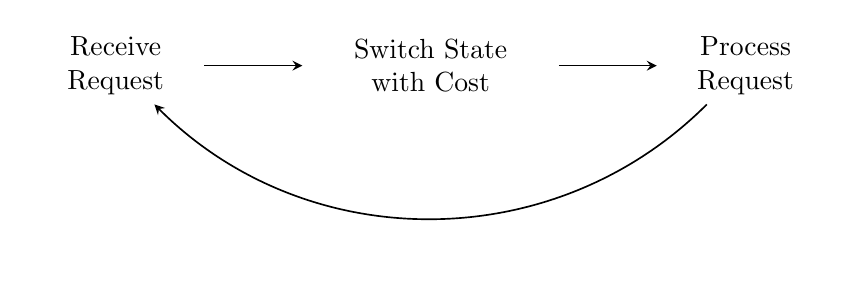
\begin{tikzpicture}[>=stealth, semithick]
                \node[align=center, text width=2cm] (0) at (0, 0) {Receive Request};
                \node[align=center, text width=3cm] (1) at (4, 0) {Switch State with Cost};
                \node[align=center, text width=2cm] (2) at (8, 0) {Process Request};
                \path[->] (0) edge (1)
                          (1) edge (2)
                          (2) edge[bend left=45] (0);
            \end{tikzpicture}
            \begin{tikzpicture}[>=stealth, semithick]
                \node[align=center, text width=2cm] (0) at (0, 0) {\(\tau_i\)};
                \node[align=center, text width=3cm] (1) at (4, 0) {\((x_{i-1} \mapsto x_i)\) with cost \(x_{i-1}x_i\)};
                \node[align=center, text width=2cm] (2) at (8, 0) {\(\tau_i(x_i)\)};
                \path[->] (0) edge (1)
                          (1) edge (2)
                          (2) edge[bend left=45] (0);
            \end{tikzpicture}
        }
    \end{figure}

    \emph{Examples:} The Ice Cream Problem \cite[pp. 74-75]{Woeginger}, the Paging Problem \cite[p. 124]{Borodin} and the \(k\)-Server Problem \cite[pp. 87-88]{Woeginger}.

    \begin{minipage}{0.33\linewidth}
        \centering
        \huge
        \begin{align*}
            \begin{array}{c|c|c}
                    & V & S\\\hline
                V_M & 1 & 4\\
                S_M & 2 & 2
            \end{array}
        \end{align*}
    \end{minipage}
    \begin{minipage}{0.33\linewidth}
        \centering
        \scalebox{0.9}{
            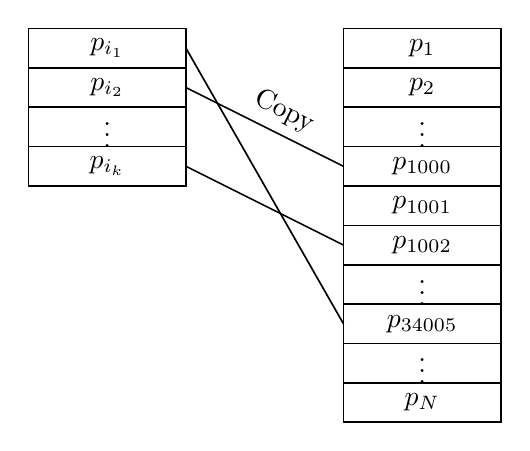
\begin{tikzpicture}[>=stealth, semithick]
                \draw (0, 0) rectangle (2, -0.5) node[pos=0.5] {\(p_{i_1}\)};
                \draw (0, -0.5) rectangle (2, -1) node[pos=0.5] {\(p_{i_2}\)};
                \draw (0, -1) rectangle (2, -1.5) node[pos=0.5] {\(\vdots\)};
                \draw (0, -1.5) rectangle (2, -2) node[pos=0.5] {\(p_{i_k}\)};
                \draw (4, 0) rectangle (6, -0.5) node[pos=0.5] {\(p_1\)};
                \draw (4, -0.5) rectangle (6, -1) node[pos=0.5] {\(p_2\)};
                \draw (4, -1.0) rectangle (6, -1.5) node[pos=0.5] {\(\vdots\)};
                \draw (4, -1.5) rectangle (6, -2.0) node[pos=0.5] {\(p_{1000}\)};
                \draw (4, -2.0) rectangle (6, -2.5) node[pos=0.5] {\(p_{1001}\)};
                \draw (4, -2.5) rectangle (6, -3.0) node[pos=0.5] {\(p_{1002}\)};
                \draw (4, -3.0) rectangle (6, -3.5) node[pos=0.5] {\(\vdots\)};
                \draw (4, -3.5) rectangle (6, -4.0) node[pos=0.5] {\(p_{34005}\)};
                \draw (4, -4.0) rectangle (6, -4.5) node[pos=0.5] {\(\vdots\)};
                \draw (4, -4.5) rectangle (6, -5.0) node[pos=0.5] {\(p_N\)};
                \draw (2, -0.25) -- (4, -3.75);
                \draw (2, -0.75) -- (4, -1.75) node[above, pos=0.56, rotate=-26.5651] {Copy};
                \draw (2, -1.75) -- (4, -2.75);
            \end{tikzpicture}
        }
    \end{minipage}
    \begin{minipage}{0.33\linewidth}
        \centering
        \scalebox{1.1}{
            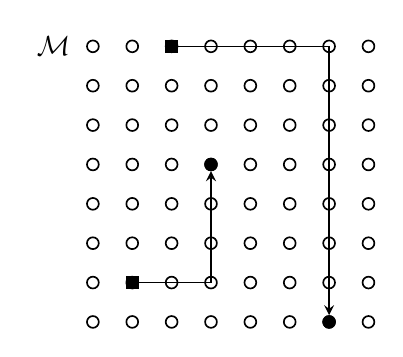
\begin{tikzpicture}[>=stealth, semithick]
                \tikzset{point/.style={draw, circle, inner sep=0pt, minimum size=1.5mm}}
                \newcommand{\dw}{0.5}
                \foreach \x in {0, 1, ..., 7} {
                    \foreach \y in {0, 1, ..., 7} {
                        \node[point] at (\dw*\x, \dw*\y) {};
                    }
                }
                \node at (-0.5, \dw * 7) {\(\mathcal{M}\)};
                \node[fill, point] (r1) at (\dw*3, \dw*4) {};
                \node[fill, point] (r2) at (\dw*6, \dw*0) {};
                \node[fill, point, rectangle] (k1) at (\dw*1, \dw*1) {};
                \node[fill, point, rectangle] (k2) at (\dw*2, \dw*7) {};
                \draw[->] (k1) -- (\dw*3, \dw*1) -- (r1);
                \draw[->] (k2) -- (\dw*6, \dw*7) -- (r2);
            \end{tikzpicture}
        }
    \end{minipage}

    \begin{definition}[{\cite[p. 76]{Woeginger}}]
        Let \(x \in \mathcal{M}^n\) be a one-indexed sequence of states. Set
        \begin{align}
            \text{cost}(x_0, \tau, x) \coloneqq \sum_{i=1}^n x_{i-1}x_i + \tau_i(x_i), \qquad \text{opt}(x_0, \tau) \coloneqq \min_{x \in \mathcal{M}^n} \text{cost}(x_0, \tau, x)
        \end{align}
        Let further \(\mathcal{T}^* \coloneqq \bigcup_{m=1}^\infty \mathcal{T}^m\). A (deterministic) \emph{online strategy/online algorithm} for \(\mathcal{M}\) is a map \(\mathcal{A}\colon \mathcal{M} \times \mathcal{T}^* \to \mathcal{M}\). We further set the cost of execution by \(\mathcal{A}\) as
        \begin{align}
            \text{cost}_{\mathcal{A}}(x_0, \tau) \coloneqq \text{cost}(x_0, \tau, \mathcal{A}(x_0, \tau_1)\mathcal{A}(x_0, \tau_1\tau_2)...\mathcal{A}(x_0, \tau_1\tau_2...\tau_n))
        \end{align}
        \(\mathcal{A}\) is called \emph{\(c\)-competitive with initial function \(\alpha\colon \mathcal{M} \to \mathcal{R}\)}, where \(c \in \mathbb{R}\), if for any \(x_0 \in \mathcal{M}\) and \(\tau \in \mathcal{T}^*\), we have
        \begin{align}
            \text{cost}_{\mathcal{A}}(x_0, \tau) \leq c \; \text{opt}(x_0, \tau) + \alpha(x_0)
        \end{align}
        Furthermore, the value \(\text{argmin}_{c \in \mathbb{R}} (\mathcal{A} \text{ is } c \text{-competitive})\), if it exists, is called the \emph{competitive-ratio} of \(\mathcal{A}\).
    \end{definition}

    \begin{definition}[Work Functions]
        The function
        \begin{align}
            \omega\colon \mathcal{M} \to \mathbb{R}, x \mapsto \textstyle\min_{(x_1, ..., x_{n-1}) \in \mathcal{M}^{n-1}} \text{cost}(x_0, \tau, (x_0, x_1, ..., x_{n-1}, x))
        \end{align}
        is called the \emph{work function} for \(x_0\) and \(\tau\).
    \end{definition}

    \newpage

    \begin{mdframed}
        \paragraph*{\textbf{Dynamic Program for Computing the Work Function}}
        Let \(\omega_i\) for any \(i \in \mathbb{N}\), \(0 \leq i \leq n\), denote the work function of \(x_0\) and \((\tau_1, ..., \tau_i)\) computing the lowest costs for the first \(i\) tasks. Then the following dynamic program allows the computation of \(\omega_0, ..., \omega_n\).
        \begin{align}
            \omega_0(x) &= x_0x\\
            \omega_{i+1}(x) &= \min_{x' \in \mathcal{M}} \omega_i(x') + \tau_{i+1}(x') + x'x \label{work_function_comp_dyn_prog_second_stmt}
        \end{align}
    \end{mdframed}

    \phantom{}

    \begin{mdframed}
        \paragraph*{\textbf{The Work Function Algorithm (WFA)}} Let \(i \in \mathbb{N}\), \(1 \leq i \leq n-1\) and suppose the states \(x_0, x_1, ..., x_i\) have already been computed. Then the WFA chooses the next state by
        \begin{align*}
            x_{i+1} &\in \arg\min_{x \in \mathcal{M}} \omega_{i+1}(x)+x_ix \tag{\(\dagger\)} \label{wfa_first_condition}\\
            \text{s.t. } \omega_{i+1}(x_{i+1}) &= \omega_i(x_{i+1})+\tau_{i+1}(x_{i+1}) \tag{\Ankh} \label{wfa_second_condition}
        \end{align*}
    \end{mdframed}

    \begin{theorem}[{\cite[pp. 132-133]{Borodin}}]
        The WFA is well-defined.
    \end{theorem}

    \begin{theorem}[{\cite[pp. 133-134]{Borodin}}] \label{wfa_competitiveness_theorem}
        The WFA is \((2N-1)\)-competitive.
    \end{theorem}
    
    \begin{theorem}[{\cite[pp. 128-132]{Borodin}}]
        The competitive ratio of any deterministic online algorithm for general MTS is lower bounded by \((2N-1)\).
    \end{theorem}

    \begin{conjecture}[{\cite[pp. 152-153]{Borodin}}]
        There exists a \(k\)-competitive deterministic online algorithm for the \(k\)-server algorithm over any metric space.
    \end{conjecture}

    \begin{table}[!hbtp]
        \begin{tabular}{c|c|c}
            Problem & \(c_{\text{WFA}}\) & \(c_{\text{Better}}\)\\\hline
            Ice Cream & \(3\) & \(7/6\) (claim in exercise, \cite[pp. 80-82]{Woeginger}) \\
            Paging & \(2\binom{N}{k}-1\) & \(k\) (tight, \cite[pp. 54-56]{Woeginger})\\
            \(k\)-Server MTS WFA & \(2N^k-1\) & See below\\
            \(2\)-Server WFA & \(2\) (tight, \cite[pp. 87-89, p. 94]{Woeginger}) & None\\
            \(k\)-Server WFA, \(k \geq 3\) & \(2k-1\) (\cite[pp. 92-93]{Woeginger}) & Open\\
            \(k\)-Server WFA, \(|\mathcal{M}| = k+2\) & \(k\) (tight, \cite[pp. 87-89, pp. 94-95]{Woeginger}) & None
        \end{tabular}
    \end{table}

    \printbibliography{}
\end{document}
